\newpage 

\section{Download Python for Desktop}

As you learn Instrumentation throughout the semester, you will be
tasked with creating computer programs on the Circuit Playground
Express (CPX). The CPX itself has it’s own RAM, CPU, HDD and many
sensors. Your CPX is kind of like a mini computer! You can plug the
CPX into your computer via USB and access the hard drive (HDD) from
your own computer. When you program on the CPX you need to write
programs on the CPX itself so that the mini computer can run the
program you wrote. The CPX knows how to read multiple different
languages but in this class we are going to write everything in the
\href{https://www.python.org/}{Python} language which has been ported
to the CPX and called
\href{https://circuitpython.org/}{CircuitPython}. Since we have to
write everything in CircuitPython we 
need to first learn how to program some things in Python. You can
easily download Python by itself but it’s nice to get what’s called an
Integrated Development Environment (IDE). This way you can practice
writing Python code on your computer while you wait for your purchases
to arrive in the mail. 

So which IDE can you download and which is recommended? I recommend
two IDEs. They are listed below. I recommend getting either one. If
you just Google “Python download” you will find a humongous list of
editors (Scratch, Anaconda, Canopy, Eclipse, PyDev, etc). It’s easy to
get lost when searching for something so broad. You’ve been warned.

\subsection{Thonny}

Thonny - \url{https://thonny.org/} -
\href{https://www.youtube.com/watch?v=qaxukpYRqfA&list=PL_D7_GvGz-v1RsDs_OdNW65qRjEjmpfQx&index=14}{Youtube
  video on how to install}

\begin{figure}[H]
  \begin{center}
    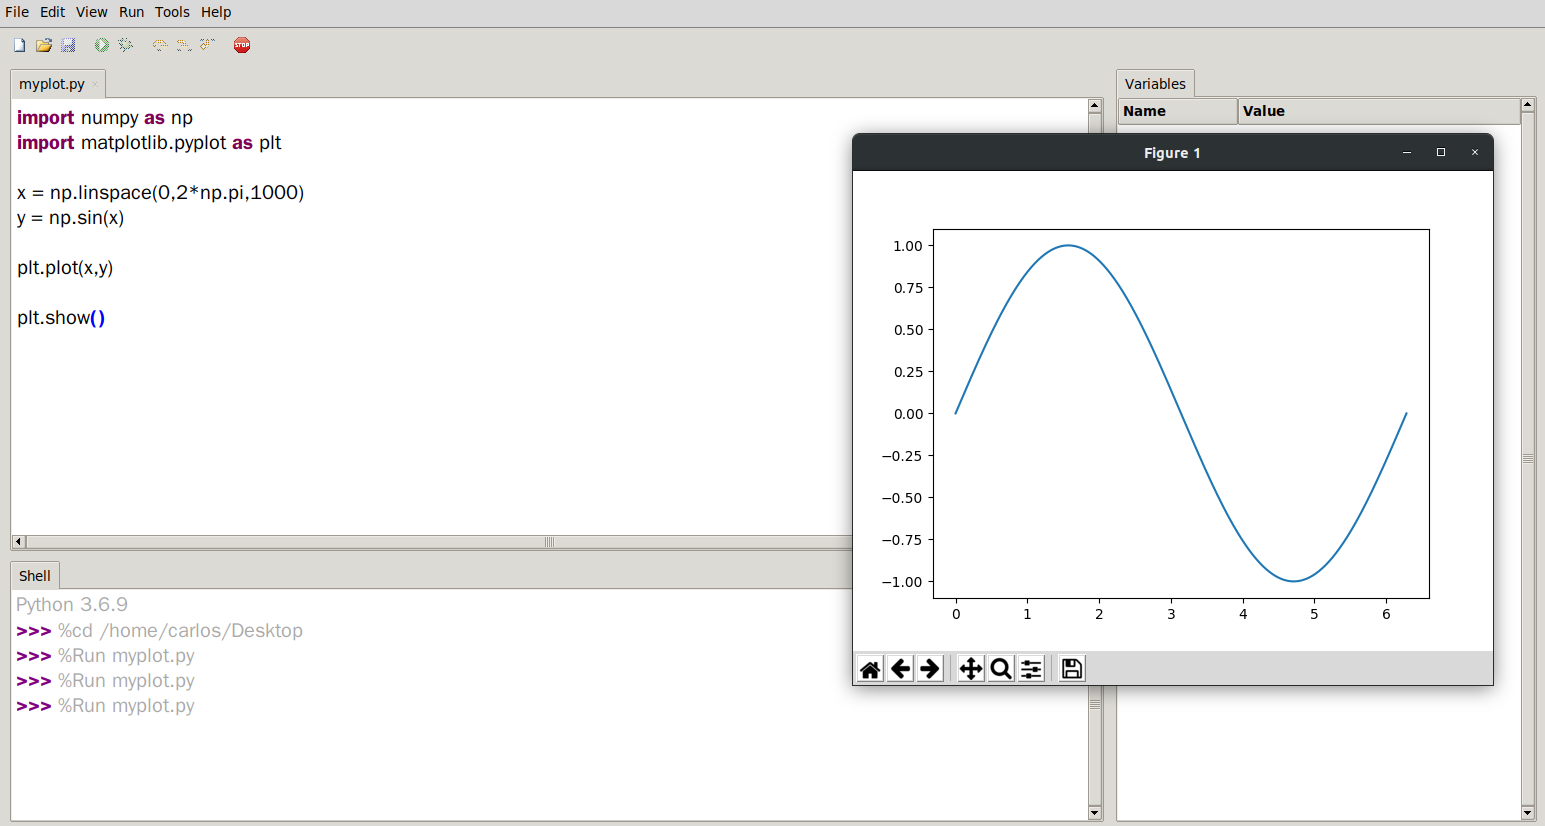
\includegraphics[width=\textwidth]{Figures/Thonny.png}
  \end{center}
\end{figure}

\subsection{Spyder}

Spyder - \url{https://www.spyder-ide.org/} - \href{https://www.youtube.com/watch?v=OjYwET-6QtE&list=PL_D7_GvGz-v1RsDs_OdNW65qRjEjmpfQx&index=35}{Youtube video on how to install}

\begin{figure}[H]
  \begin{center}
    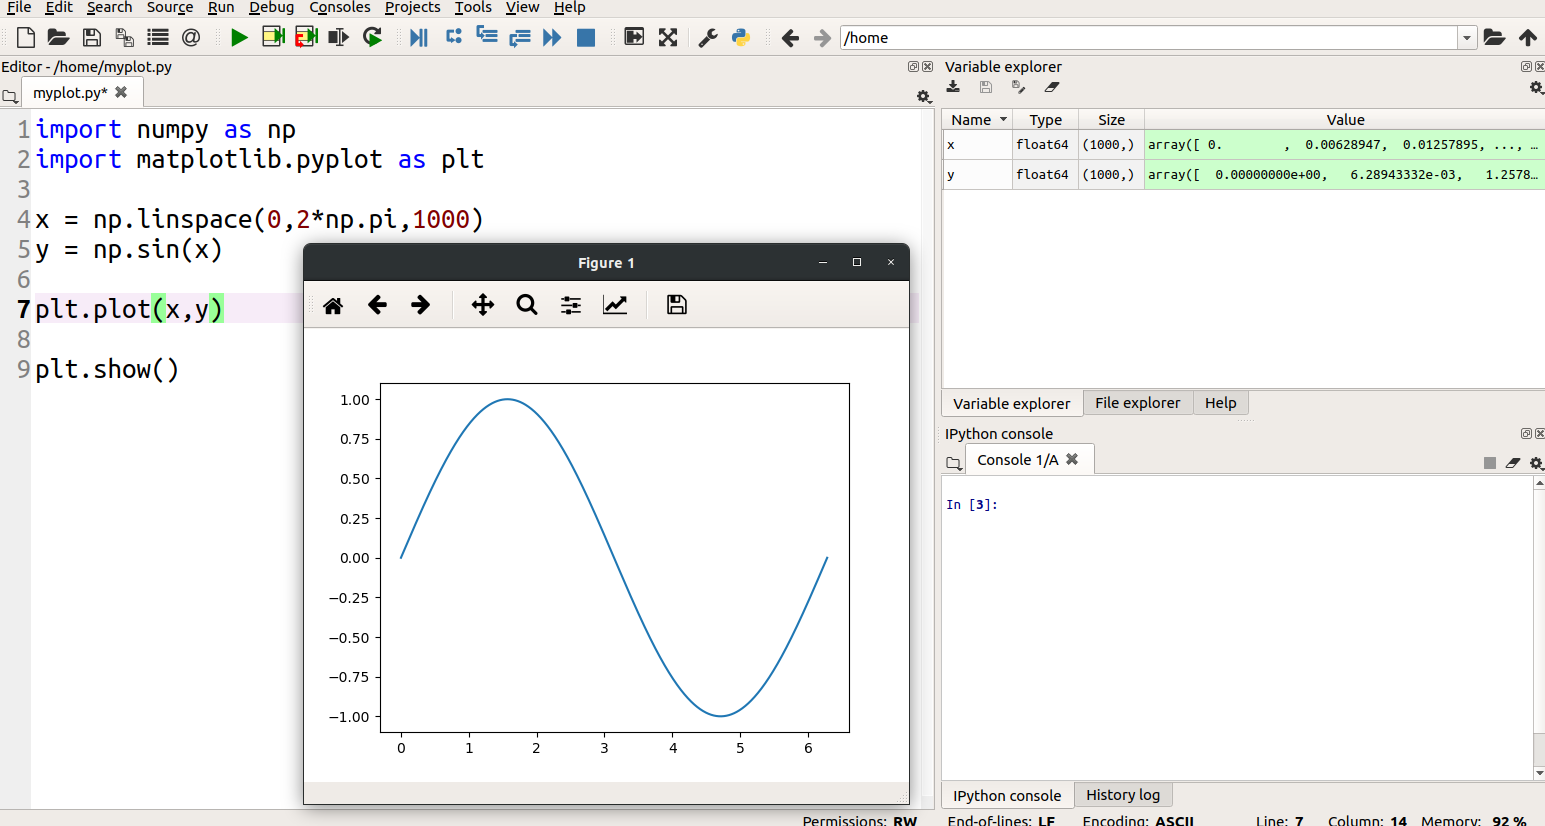
\includegraphics[width=\textwidth]{Figures/Spyder.png}
  \end{center}
\end{figure}

\subsection{Other Options}

It is possible to use
\href{https://colab.research.google.com/drive/1-VzSDojevQZ6A0oJNol9YXV6SRp3FKeP}{Google
  Colab} if you want to collaborate on Python projects or even get apps for your phone (\href{https://play.google.com/store/apps/details?id=ru.iiec.pydroid3&hl=en_US&gl=US}{Pydroid} or \href{https://apps.apple.com/us/app/pythonista-3/id1085978097}{Pythonista}
depending on Android or iPhone). You'll need to download 32 bit or 64
bit but which one? Well you need to figure out how many bits your
computer has. This is a great thing to Google. Type the following: "do
I have a 32 bit or 64 bit computer" into Google. I’m willing to bet
you have a 64 bit computer but you may as well check. We’ll learn
about the difference between 32 and 64 bit computers when we get to
the projects on Binary.

\subsection{Setting up your IDE}

Once you have Thonny or Spyder installed you need to install numpy and
matplotlib which are modules within Python that allow us to do some
extra things like numerical computation with Python (numpy) and Matlab
style Plotting libraries (matplotlib). I explain how to install
modules in my Youtube videos above; however, you need to head over to
Tools>Manage Packages in Thonny. You can see in the image below I
already have version 3.1.2 but I can upgrade to 3.2.2

\begin{figure}[H]
  \begin{center}
    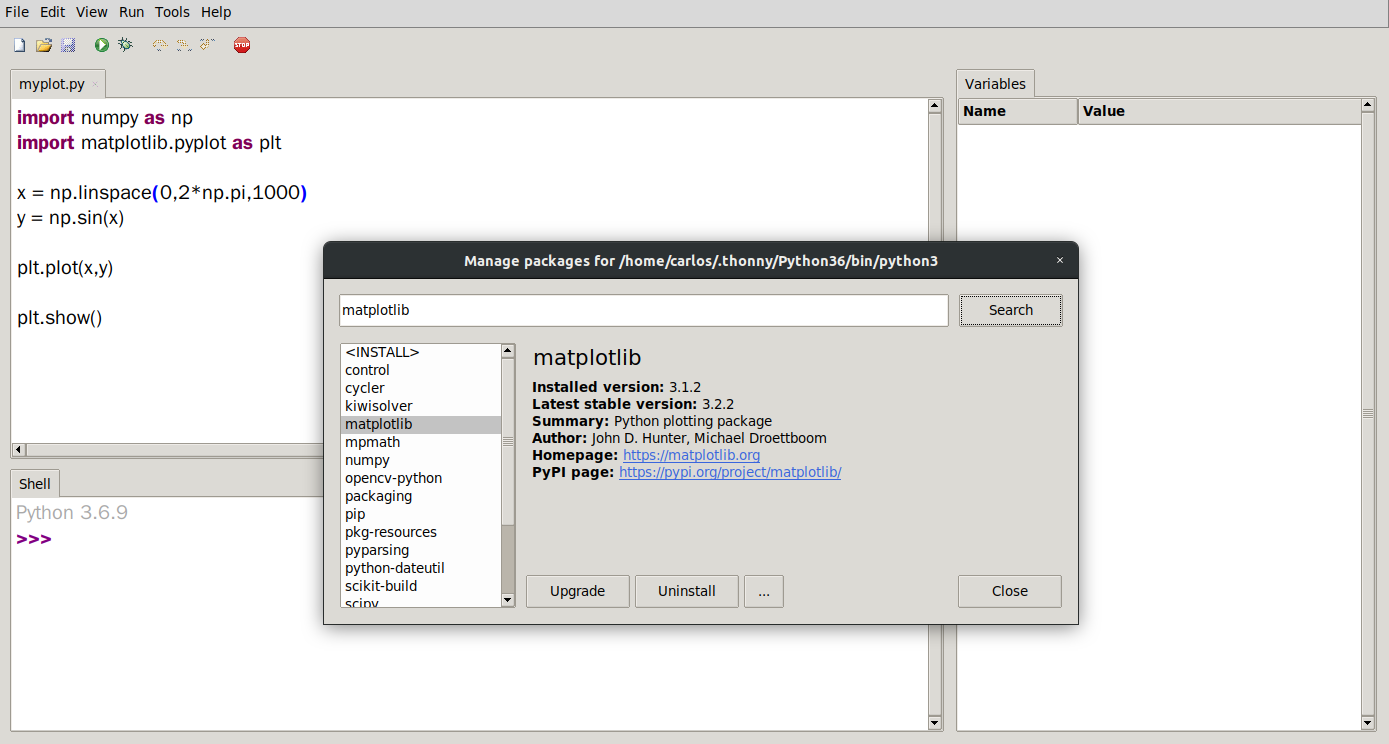
\includegraphics[width=\textwidth]{Figures/IDE_upgrades.png}
  \end{center}
\end{figure}

If numpy or matplotlib is not already included in Spyder then you need
to type the following into the Python Console in the lower right hand
corner of Spyder which is called the IPython console. 

\begin{verbatim}
!pip install matplotlib
\end{verbatim}

If that doesn’t work try

\begin{verbatim}
!pip3 install matplotlib
\end{verbatim}

You can see in the output example below that I already have matplotlib
installed as it says “requirement already satisfied”. Assuming you
have a valid internet connection it will install the necessary
module. 
\begin{figure}[H]
  \begin{center}
    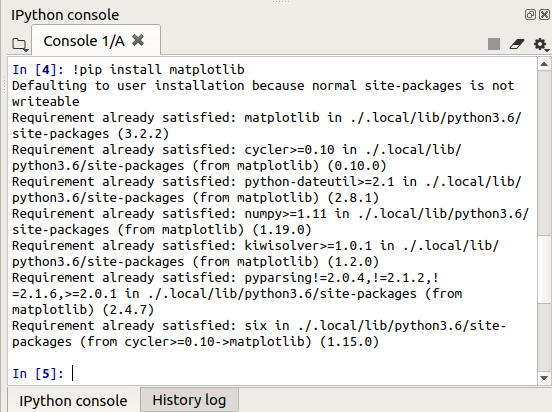
\includegraphics[width=0.5\textwidth]{Figures/console_thonny.png}
  \end{center}
\end{figure}

\subsection{Scripting}

Once you have numpy and matplotlib it’s time to make a plot. I have a
pretty \href{https://www.youtube.com/watch?v=7nAzHPURYW0&list=PL_D7_GvGz-v1RsDs_OdNW65qRjEjmpfQx&index=8}{comprehensive youtube video on how to plot in matplotlib} but if
you prefer text I will walk through a simple example.

\begin{figure}[H]
  \begin{center}
    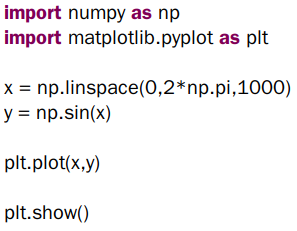
\includegraphics[width=0.5\textwidth]{Figures/matplotlib_example.png}
  \end{center}
\end{figure}

The code above will plot a sine wave from 0 to 2pi. The two lines at
the top are importing the numpy and matplotlib modules you installed
earlier. When they are imported we give them shorter names so it’s
easier to reference them so numpy will now be called np and
matplotlib.pyplot will be called plt. The next two lines then create a
vector “x” from 0 to 2pi using 1000 data points. The next line then
uses the sine function to create the vector “y”. Finally “x” and “y”
are plotted and the figure is instructed to pop up on your screen
using the show() function.


%% Now that you somewhat understand some of
%% this I’d like you to plot the following function: 

%% \begin{equation}
%%   T(t) = 60(1-e^{-5t})+30
%% \end{equation}

%% Plot the function from 0 to 10 seconds and label the x axis ‘Time
%% (sec)’ and the y-axis ‘Temperature (F)’. Add a grid as well. There are
%% some things that I have not explicitly shown you how to do. The reason
%% why is because I want to teach you how to fish for information.  

%% The first thing I recommend trying is to type in the commands in the
%% IPython console or the Shell. Type the first two commands below which
%% will show you every single function that numpy has available to you. 
%% \ \\

\subsection{Built-In Help Function and dir()}

Running code will always create syntax errors. Typing your syntax
error into Google will yield so many results you might get
lost. Sometimes it helps to know how to learn things just from your
computer. For example, type in the commands below in the IPython
console or the Shell.

\noindent {\it import numpy as np}\\
{\it dir(np)}
\ \\

\begin{figure}[H]
  \begin{center}
    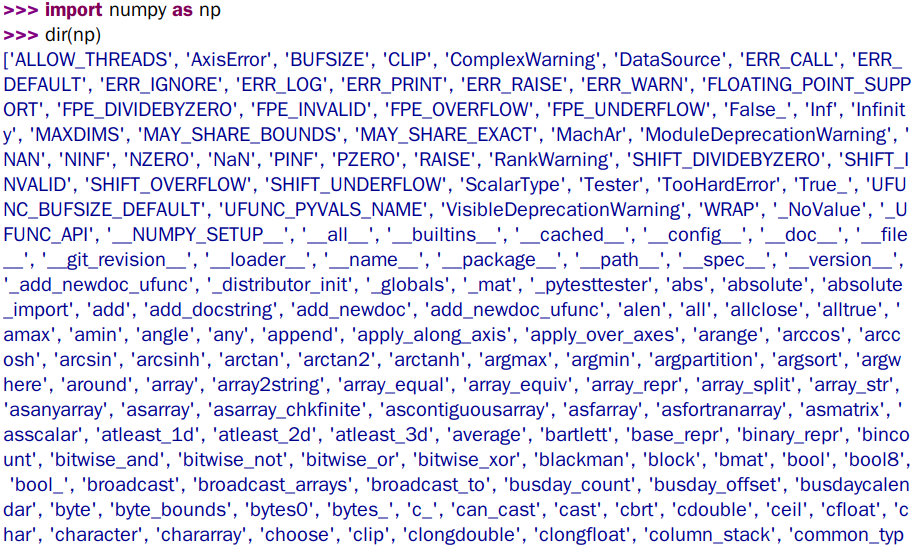
\includegraphics[width=\textwidth]{Figures/dir.png}
  \end{center}
\end{figure}

I included a photo of the output from the dir function. You’ll notice
there are a ton of functions in numpy. Every function in Python has a
\begin{verbatim} 
__doc__
\end{verbatim}

function. That’s two underscores followed by “doc” and then
another two underscores. If you’re ever curious about what a
particular function does you can just run the command below again in
the IPython console or Shell. In this example I’m looking at what
{\it arctan2} does.  

\begin{verbatim}
print(np.arctan2.__doc__)
\end{verbatim}

\begin{figure}[H]
  \begin{center}
    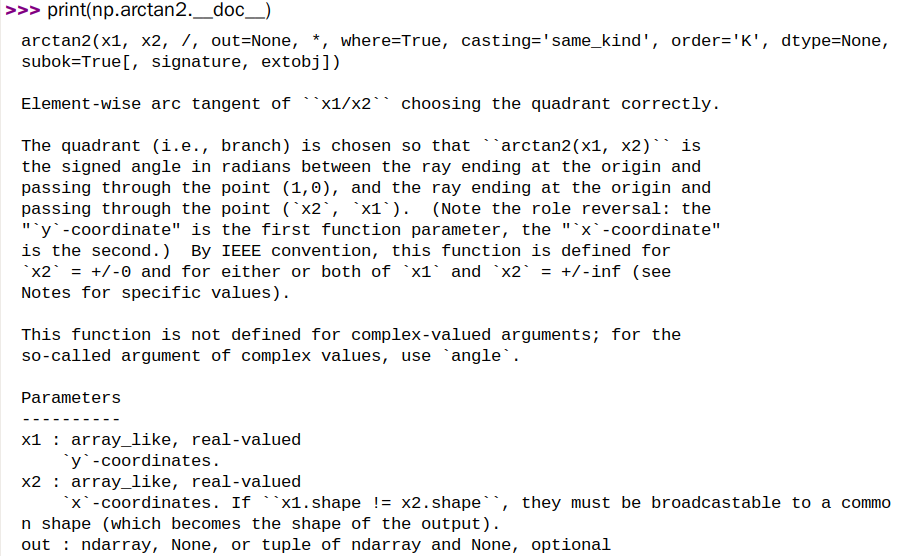
\includegraphics[width=\textwidth]{Figures/arctan2_doc.png}
  \end{center}
\end{figure}

You’ll see that arctan2 takes 2 input arguments “x1” and “x2”. I
didn’t include the entire output but if you continue to scroll through
the output it will even include examples on how to use the function.  

Another way to learn certain functions is by visiting the appropriate
documentation. The \href{https://numpy.org/doc/}{Numpy Docs} website
for example has all the documentation you need for Numpy. Navigating
that website you can find the same \href{https://numpy.org/doc/1.19/reference/generated/numpy.arctan2.html?highlight=arctan2#numpy.arctan2}{documentation for arctan2}.

As a last resort you can always Google “how to compute the inverse
tangent 2 function in Python”. Note though that there is so much
content out there on Google that you could easily get lost. Still,
there’s also so much information that the answers are out there for
just about anything.  

So you have three methods for finding out how to program in
python. The dir and {\it \_\_doc\_\_} functions in Python, using the appropriate
documentation online and of course Google. I’m lumping Youtube in with
Google which is also another way to learn information although when I
want to find information quickly I just use the documentation. It’s
the best in my opinion. 

\subsection{Assignment}

Your assignment for this project is to plot the equation below from 0 to 10 seconds and include that Figure in your report. You must add a grid and label the x-axis ‘Time (sec)’ and the y-axis ‘Temperature (F)’

\begin{equation}
  T(t) = 60(1-e^{-5t})+30
\end{equation}

Once you've completed the project above, upload a PDF with all of the photos and text
below included. My recommendation is for you to create a Word document
and insert all the photos and text into the document. Then export the
Word document to a PDF. For videos I suggest uploading the videos to
Google Drive, turn on link sharing and include a link in your
PDF. Note that all code must be included in the appendix or you'll be
penalized 10\%. 


\begin{enumerate}[itemsep=-5pt]
  \item Include a screenshot of your Python IDE (Thonny or Spyder is suggested) - 40\%
  \item Include the plot of temperature vs time being sure to save the figure so it is in high resolution - 40\%
\end{enumerate}
